% REMEMBER: You must not plagiarise anything in your report. Be extremely careful.

\documentclass{l4proj}

    
%
% put any additional packages here
%

\begin{document}

%==============================================================================
%% METADATA
\title{Exploring using MeSH tags for Literature Based Discovery}
\author{Timothy R Baldock}
\date{March 22, 2024}

\maketitle

%==============================================================================
%% ABSTRACT
\begin{abstract}
    
    It is increasingly difficult for researchers to keep up with the rate at which research is being published. In this project I have tested  machine learning techniques for the automated capture of literature content and prediction of potential scientific development to support the researcher to develop research hypothesis. In particular, in this project I investigated using a knowledge graph of PubMed MeSH tags to enable link prediction of potential connections between biomedical concepts. Three prediction systems; Swanson's ABC system, a graph neural network and matrix factorisation, were compared and combined to explore how this data can be used for literature based discovery. The results established that the most effective  system was the implementation of Swanson's ABC system, although the combination of this and the graph neural network showed promise at being able to extract additional information. 

\end{abstract}


%==============================================================================

% EDUCATION REUSE CONSENT FORM
% If you consent to your project being shown to future students for educational purposes
% then insert your name and the date below to  sign the education use form that appears in the front of the document. 
% You must explicitly give consent if you wish to do so.
% If you sign, your project may be included in the Hall of Fame if it scores particularly highly.
%
% Please note that you are under no obligation to sign 
% this declaration, but doing so would help future students.
%
\def\consentname {Timothy R Baldock} % your full name
\def\consentdate {22 March 2024} % the date you agree
%
\educationalconsent


%==============================================================================
\tableofcontents

%==============================================================================
%% Notes on formatting
%==============================================================================
% The first page, abstract and table of contents are numbered using Roman numerals and are not
% included in the page count. 
%
% From now on pages are numbered
% using Arabic numerals. Therefore, immediately after the first call to \chapter we need the call
% \pagenumbering{arabic} and this should be called once only in the document. 
%
% Do not alter the bibliography style.
%
% The first Chapter should then be on page 1. You are allowed 40 pages for a 40 credit project and 30 pages for a 
% 20 credit report. This includes everything numbered in Arabic numerals (excluding front matter) up
% to but excluding the appendices and bibliography.
%
% You must not alter text size (it is currently 10pt) or alter margins or spacing.
%
%
%==================================================================================================================================
%
% IMPORTANT
% The chapter headings here are **suggestions**. You don't have to follow this model if
% it doesn't fit your project. Every project should have an introduction and conclusion,
% however. 
%
%==================================================================================================================================
\chapter{Introduction}

% reset page numbering. Don't remove this!
\pagenumbering{arabic} 

\section{Motivation}

\subsection{Increasing Research Rate}

The global research rate is increasing. This is in part fuelled by the global spending on research and development that has increased to 2.4 trillion dollars in 2020 from only 675 billion in 2000 as reported by the Congressional Research \cite{congress} (2022). As research across the world continues to grow, so too does our accumulated knowledge grow. According to \cite{bornmann_growth_2015}, the rate of research increased exponentially between 1980 and 2013, with a growth rate of about 3\% \textit{per annum} for global scientific publications in this time frame. With an ever-growing repository of information it becomes more difficult to accumulate expertise in a field. This is further exacerbated by the increasing rate of research which also makes it even more difficult for individual experts to stay up to date with developments in their field. \\ 

The result of this, is a narrowing of expertise as discussed by \cite{swanson_fish_1986}. To become expert in a field requires increasingly more time to be spent on a narrower area of research. A consequence of this is that individuals can benefit less from their wider understanding of their field as not only can they spend less time learning about the broader subject but also the required time taken to properly develop knowledge in other parts of their subject increases.\\ 

\subsection{Literature Based Discovery}

Literature based discovery (LBD) seeks to address this issue by creating predictive systems to identify undiscovered links that might be worth exploring. The existence of such undiscovered links was established by \cite{swanson_fish_1986}, when he determined that fish oil relieved Raynaud's Syndrome. His discovery system used the connection between dietary fish oil reducing blood viscosity and that high blood viscosity exacerbates Raynaud's Syndrome to propose a link between the two. Prior to this, fish oil had not been discovered as a treatment for Raynaud's Syndrome, despite all the necessary linking research already existing. Therefore, his system of LBD enabled the discovery this treatment. \\

There could be many similar connections between concepts like this, in clinical and biological research, that have never been discovered, because the right combination of papers have not been read together by the right person. Many different systems have been designed and implemented to approach identifying these links. These systems can vary in what data they use to represent these concepts, how they try to define connections and how they rate different connections to scoring, sorting and evaluation. \\

\section{Aims}

This project aims to explore how MeSH tags \citep{mesh_home}, a labelling system for biomedical research papers, can be used for LBD. First, this project will create a knowledge graph to represent the co-occurrence of MeSH tags in articles. The resources used in other research is not available for this project, so this project will not seek to compare results with external results. Instead, this project will implement a selection of systems using this knowledge graph to compare how they perform, and determine which makes the most accurate predictions using this data. Furthermore, the combination of these systems will be explored to see if this can improve the predictions and extract further insights from the data. \\ 

%==================================================================================================================================
\chapter{Background}

\section{Literature Based Discovery}

LBD is the idea that we can use the vast and growing database of research to generate hypothesis for future work. The work done by \cite{henry_literature_2017}, provides many examples of LBD's applications and achievements including identifying potential treatments for cancer and finding treatments for cataracts. Biomedical research is the field in which LBD is most utilised, but there are numerous instances of its use in other fields. LBD is also used beyond biomedical research, for example the oceanographic climate science by \cite{aamot_literature-based_2014} is a case of LBD being applied to another field with its application in studying climate change. Given the increasing quantity and funding of research, being able to effectively generate hypothesis by linking different areas of expertise will only become more important.\\  

\section{Knowledge Graph}

One way to represent this data is as a knowledge graph. These represent data by defining it as a series of entities and relationships. For example, a family could be represented this way as seen in \Cref{fig:knowledge_graph}, with the members as nodes in the graph and their relationships as edges. More information could be added here too, maybe the time they've had this relationship could be added to each edge, or the height of the member could be added to the node. In this way, can a wide array of data be represented in a standardised system that has common rules and features. If a graph has multiple types of edges, as in \Cref{fig:knowledge_graph}, or multiple types of node, like if each person was categorised male or female, then a graph is heterogeneous. If a graph has only one type of node and one type of edge then instead it is homogeneous. This type of graph can still have values attached to the edges as weights, but it cannot attach further labels without becoming heterogeneous. \\ 

\begin{figure}[h]
    \centering
    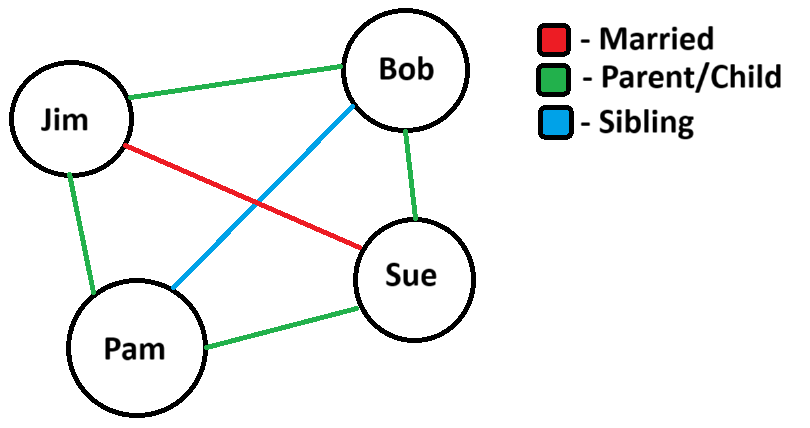
\includegraphics[width=0.6\linewidth]{images/knowledge_graph.png}
    \caption{Example knowledge graph of a family}
    \label{fig:knowledge_graph}
\end{figure}

\section{Link Prediction}

TO utilise this data structure for this problem, What does LBD mean in the context of a knowledge graph. LBD seeks to discover links between concepts that have sound logic as to why they might exist but have not yet been explored or proven yet. Concepts should therefore be represented as nodes and if there is a connection between these concepts, then an edge should exist between the nodes in question. An LBD system will then seek to use the information contained in the graph to predict new edges, that do not exist in the graph but might actually exist between the concepts. A notable feature of these link prediction systems is that predicted edges that do not exist yet are not necessarily wrong, they are just undiscovered as of yet. However, when evaluating link prediction systems, a system that successfully guesses more existing edges is therefore a system that can be trusted to better evaluate non-existing edges. These features of link prediction therefore pose three key problems for systems to address: \\

\begin{itemize}
    \item \textbf{Nodes,} what constitutes a concept, and what further information about them should be attached to the node.
    \item \textbf{Edges,} how to establish a relationship between two concepts, and how to determine if that relationship is meaningful or not.
    \item \textbf{Predictions,} How to use the information of these nodes and edges to make predictions about what new edges would be worth researching. \\
\end{itemize}

There is much existing research that explores these points. Although not all of this research uses knowledge graphs to structure the data, the approaches taken to defining concepts, establishing relationships between them and making predictions on undiscovered relationships is crucial to developing a system for this project. \\

\section{Discovery Methods}

\subsection{Swanson's ABC System}

\begin{figure}
    \centering
    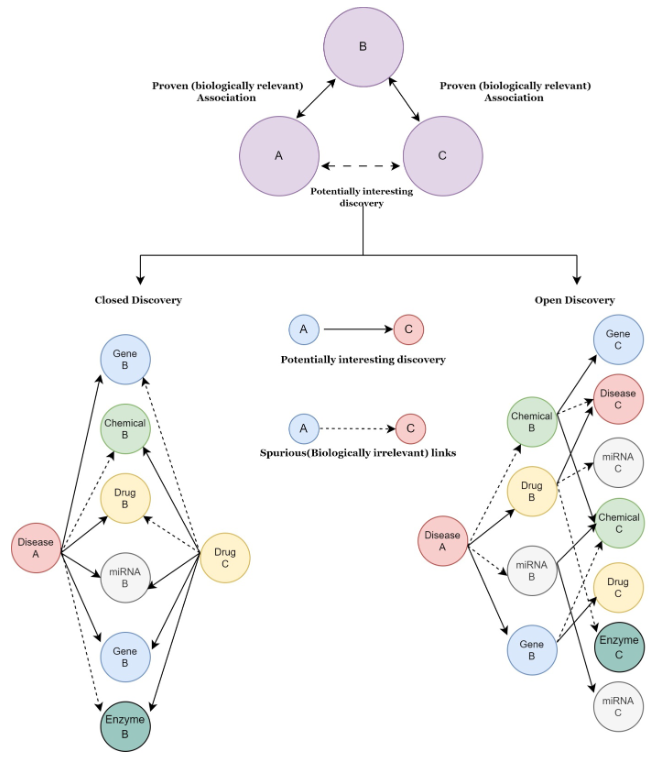
\includegraphics[width=\linewidth]{images/abc_open_closed.png}
    \caption{Examples of ABC connections, Open discovery and Closed discovery. \citep{bhasuran_literature_2023}}
    \label{fig:open_closed}
\end{figure}

LBD is founded on Swanson's ABC approach. In this approach, if concepts A and B have an established relationship, and concepts B and C do too, then there may well be a transitive relationship between A and C. This is visualised at the top of \Cref{fig:open_closed} where A and B, and B and C are linked by proven association and so the link between A and C might be a potentially interesting discovery. In particular, this system is interested in circumstances where no relationship between A and C has been previously established as this might therefore be a new connection that could be discovered. An example of this being successfully implemented by Swanson himself would be his discovery of using fish oil to treat Raynaud's syndrome. \\

\subsubsection{Open Discovery}

Open and closed discovery are the two main methods of Swanson's ABC system. Open discovery involves the user to have an identified concept A for which to discover possible C concepts. This can be done by identifying all the possible C concepts that are not linked to the original A but have at least one B concept in common with A. The connection between A and each C can then be evaluated by some metric and used to sort the possible C concepts in some way so that they can be returned to the user in meaningful manner. In this way, Open discovery can be used to answer the questions of what concepts are connected indirectly to a given concept and how they might compare to each other. \\

\subsubsection{Closed Discovery}

Closed discovery, on the other hand, seeks to answer entirely different questions. This system requires pre-given A and C concepts so that the B connections between them can be discovered. This allows the user to check if any common ground can be found between two concepts that they might suspect have a connection. This could even be generalised beyond unconnected concepts, it could be used to explore new ways two concepts, that have pre-existing connections, might be overlapping. Closed discovery therefore asks the question of how or why two concepts are connected. The two concepts do not have to exist in isolation of each other. In fact, since they answer very different questions they can be used in combination with each other to first discover new connections and then to explore why those concepts are connected. In this way Swanson created an effective and comprehensive approach to LBD, laying the groundwork for the development that followed. \\ 

\subsection{Arrowsmith}

An example of the closed discovery system is Arrowsmith \citep{swanson_interactive_1997}, a search system created by Swanson. Arrowsmith allows the user to input two terms, which will be the A and C terms for the closed discovery. It searches these titles for terms A and C, and returns a file for each respective term containing all of the titles with that term. The next step is for the Arrowsmith software to compare the two files and create a list of all 'B' terms that appear on both files. From here a stop word list of the 5000 most common terms is used to filter out the obviously redundant words from the list. \\

In this way, Arrowsmith defines concepts as any term in an article title, and relationships between terms as co-occurrence of them in a title. This means that Arrowsmith does not have to decide what does or does not constitute a medical concept, but therefore does require the user to have sufficient knowledge to do this themselves. By using only titles, Arrowsmith avoids having to search full bodies of texts, but so does also miss any concepts not included in the titles. As it is closed discovery, it does not need to make predictions, but instead only provide a list of the linking concepts between the two provided. \\

\subsection{Bio-sbKDS}

Another approach to LBD is utilising semantic relations to create more meaningful predictions. Bio-sbKDS \citep{hu_semantic-based_2005}, Biomedical Semantic-based Knowledge Discovery System, is a system that uses biomedical ontologies to try to further automate the process of evaluating predictions. This system uses the MeSH tags of articles, a system of labels that are explained in greater detail later to represent the concepts in a paper. The focus of this system is to try to better define relationships between concepts than just the co-occurrence of them. It uses the Unified Medical Language System \citep{umls}, a system for unifying and standardising biomedical vocabularies, to categorise what the relationship between two concepts is. For example, drug A might treat symptom B, whereas if drug A and drug B are connected, then it is not the case that one treats the other, as neither is a condition. \\

This system takes in a starting concept, and a desired relation from the user. Using the UMLS, it then establishes the semantic type of the concept and the desired relationship and uses this to filter down the list of target concept types it should search for. First, it takes all articles in a desired date range that include the starting concept. Next, it searches these articles for any occurrences of concepts that fit the target concept type. These concepts are used as the connecting B terms in Swanson's work and are ranked according to how many times they are found. Next all articles in the user's desired date range are searched for the highest ranking few of these B terms. Articles with the starting term are excluded, as this system wants to find new connections. From the returned articles, the MeSH tags filtered by if they fit the required semantic type and if they are in the top 100 MeSH terms and so are deemed too common. The remaining terms are then organised by how frequently they occur. \\

In this way, Bio-sbKDS uses MeSH terms to represent concepts, and the semantic types of these terms to categorise them. By using the additional information of these categories, the system can define types of relationships between concepts and filter by these types to make more meaningful and interesting predictions as an open discovery system. \\ 

\subsection{Graph Neural Network}

In data science, machine learning has grown in use for extracting insights from especially large and complicated datasets. This is due to the inability of traditional algorithms ability to effectively run on such data, and understand all of its features. In LBD, it has been implemented in a number of different ways to make predictions of possible links between concepts. \\

One such approach to using machine learning for LBD is a Graph Neural Network (GNN). The objective of a graph neural network (GNN), is to try to learn hidden or general information implied by the graph that is not obvious to see. For example, given a set of movies that a user likes, predicting what would be other movies they would want to watch. Traditionally this would be done by categorising movies into genres, so that if a user watches a lot of action movies, then the system would recommend other action movies. However, GNNs can pick up on more subtle information, maybe users who like movies A, B and C also tend to like movie D from an entirely different genre. This allows systems to propose much more focused, accurate, and personal recommendations to users than previously. \\

GNNs do this by representing the graph as an edge vector where each edge is represented as a pair of numbers, representing the nodes joined by the edge. The node identifying numbers are embedded as each edge is processed the relevant node features are aggregated and then passed to the next layer. Using these node features, the system makes predictions about the state of each edge and compares this to the truth of if the edge exists. This result then updates the loss function and the model's understanding of the graph. This process continues over the graph and is then repeated for a number of epochs, depending on the system itself. With this information, the graph can evaluate new, unseen edges between these nodes and make a prediction on if they exist or not. \\

An implementation of such a system for LBD was done by Ding and Jin, where they implemented such a system to try to improve on the more traditional approaches to making predictions in LBD. One advantage of this system that they hoped would improve predictions was the GNNs ability to capture the implicit graph structure in its training. Another, was how the system learns to score hypothetical edges as it trains, rather than having to do this in separate stages. The idea was that with advantages like these, they would be able to optimise the prediction process for LBD. They found that in fact this system did produce better results than other systems such as word2vec, supporting their hypothesis that the advantages of a GNN system, would improve predictive capabilities of an LBD system. \\

\subsection{Matrix factorisation}

Matrix factorization is a technique in machine learning and linear algebra often used for recommendation systems. At its core, matrix factorization involves decomposing a matrix into a product of two or more matrices, with the goal of revealing hidden patterns or structures within the data. For each pair of objects, say nodes on a graph, the system will take the dot product of each objects embedding. This dot product is then compared to the truth of the relationship between the objects, for example if there is an edge connecting them on the graph. The system aims to get the dot product of each of these combinations as close to the truth of them as it can and updates the loss function of these calculations, and as it goes. In this way, the system refines the embedding of each object to maximise the similarity to the truth of the matrix across the whole of it. This can be represented as an equation as follows :\\

\begin{center}
    $\text{min}_{U,V\in \mathbb{R}^{m\times d}}\left (||A - UV^T||_{F}^{2}\right )$
\end{center}

If applied to a knowledge graphs the values can be interpreted as follows: $A \in \mathbb{R}^{m\times m}$ is the matrix of edges between nodes, the matrix learns from an embedding of nodes $ \in \mathbb{R}^{m\times d}$. $U$ and $V$ are taken from this embedding for the required nodes for each edge. 

\begin{figure}[h]
    \centering
    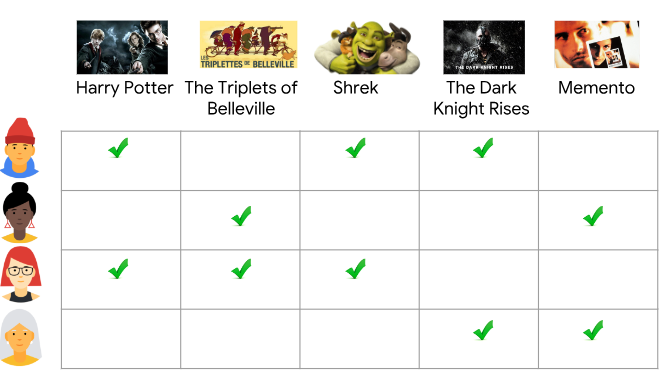
\includegraphics[width=\linewidth]{images/matrix_fact_example.png}
    \caption{image from: https://developers.google.com/machine-learning/recommendation/collaborative/matrix}
    \label{fig:matrix_fact_example}
\end{figure}

A common application of matrix factorization is collaborative filtering in recommendation systems. Here the matrix represents users' ratings for items (e.g., movies or products) as seen in \Cref{fig:matrix_fact_example}. This is an example of binary data in matrix, a user either likes or does not like a movie. However this system can also be used for more complicated relationships such as a rating. There is the limiting factor of the relationship must be represented as a singular numeric value, you could not have a matrix of text reviews, or set of numbers without first reducing them down to a single value. By decomposing this matrix into two lower-dimensional matrices, representing users and items, the algorithm can identify latent features that capture users' preferences and item characteristics. This allows for predicting missing ratings and generating personalized recommendations for users. \\

Researchers have not explicitly applied this system to LBD, however it would be a good way to bridge the gap between simple algorithmic approaches and GNNs. It can be very difficult to determine what factors are causing outcomes in a GNN, and so a matrix factorisation system can allow for a more transparent approach to making predictions on a knowledge graph. In this way could further understanding of how this data can be best used be developed. \\ 

\section{Data}

Whatever system is used, it has to utilise some data source to construct its system of concepts and relationships. often used as a foundation for this in biomedical research is PubMed, a system to help with the organising and searching of life science and biomedical literature. It was created by the National Center for Biotechnology Information and contains the abstract and other key information of over 36 million publications. The primary feature of PubMed is MEDLINE, a system containing citations from selected journals and articles indexed by MeSH tags. \\

\subsection{MeSH Tags}

MeSH tags are a system of labels used to identify and categorise biomedical articles in the PubMed database. MeSH tags provide a standardized set of terms to describe the subject matter of articles. This ensures consistency in indexing and searching across different databases and publications and is controlled by the National Library of Medicine. They were made publically available in 1996 and have been key to searching and organising biomedical literature since. By keeping the scope of terms controlled, the National Library of Medicine can ensure that similar concepts are labelled in a consistent manner, irrespective of different cultures and languages across the world. This is very important in a globally researched subject to establish a standard format to research categorization. The MeSH database is regularly updated and expanded to reflect advances in biomedical research and changes in terminology. New terms are added, and existing terms are revised to ensure accuracy and relevance in a continuously evolving field. \\

\begin{figure}[h]
    \centering
    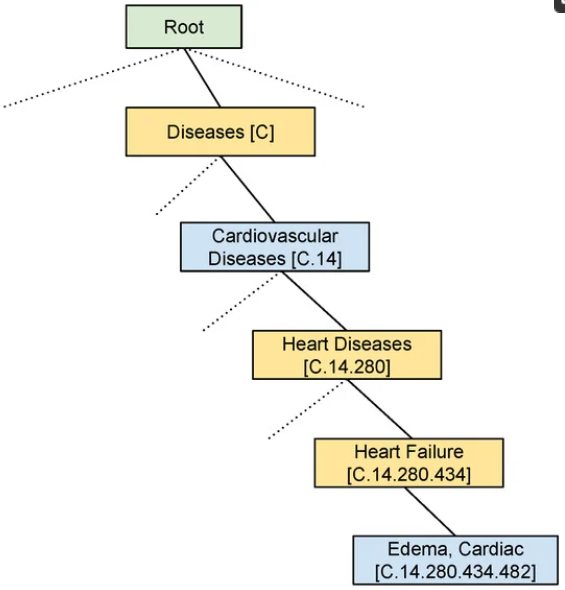
\includegraphics[width=0.6\linewidth]{images/mesh_label.png}
    \caption{image from: Integrating PubMed Label Hierarchy Knowledge into a Complex Hierarchical Deep Neural Network}
    \label{fig:mesh}
\end{figure}

In \Cref{fig:mesh}, the MeSH tag system can be seen as a hierarchical tree structure. This means that all tags are linked to broader definitions of them, so that similar types of tags can be grouped together and categorised. For example, the term "Diseases" is a broad category, under which you may find more specific terms like "Cardiovascular Diseases" and so on. This is the system that was utilised by Hu \textit{et al.} to determine the semantic types of each tag when developing their system. By providing these categories built into the tag structure, they can be used this way to automatically label data, addressing a significant problem in natural language processing (NLP). Data labelling is often required in classification problems, where a system attempts to determine what category an abject might belong to. However, fields like biomedical science would require an expert to accurately understand and label data. This would be a very time consuming task, and so would cost a lot of money to pay an expert to complete. The structure of these MeSH tags bypass the need for this step and so are a very cost effective data source in this regard.\\

Furthermore, MeSH tags reduce entire medical articles down into a small selection of key terms that best describe it. Since they are a controlled vocabulary, they ensure that papers that overlap in an area will be labelled consistently with each other. Furthermore, they are explicitly labelled by experts and so have a great value as accurate and useful data. For a field like biomedical science, that is so complicated, this is a crucial factor for LBD research and development, as can be seen in the previously discussed papers that  have used these tags. \\

MeSH tags are very efficient as data. They can be used to filter massive documents of text down into a handful of key terms that best describe the document. This will therefore save researchers using them a significant amount of time that is normally spent filtering data down into something meaningful, and since these terms are carefully selected by experts, reduce the risk that the filtering might remove vital information from the data. Furthermore, MeSH tags can be filtered down further, either by only selecting tags from certain branches of the tree, or by only using major topic tags, that are used to represent the main focus of a paper. \\

\subsection{Other Data}

Despite these benefits, MeSH tags do have drawbacks when used as data in this way. Since they are primarily tags for searching and categorising research papers, they are selected with this in mind. Information that is not deemed relevant for someone searching for this paper will therefore not be included in the MeSH tags. They are not selected to cover all areas of a paper for the purpose of LBD and so might not include information that actually could have helped identify links between research. \\
 
Because of this, there is extensive research in the field of LBD in Biomedical science that either uses more than just MeSH tags or does not use them at all. This paper has already covered Swanson's Arrowsmith system, but there is much other research that seeks to represent the concepts in a different manner. For example, the work done by Lever \textit{et al.} uses the abstracts and titles of papers, as well as some full text bodies, to determine and represent their contents. The system they built aimed to utilise the global features of a knowledge graph through singular value decomposition (SVD). As previously mentioned, they build this knowledge graph using the abstracts and titles of papers. To reduce these passages into concepts that could be used as nodes, a word list to search for was derived from desired semantic groups in the UMLS Metathesaurus (version 2016AB) such as Anatomy or Chemicals and Drugs. If a pair of these desired terms would both appear in a sentence together, then they would be deemed to be connected. In this way, this paper establishes concepts using the UMLS Metathesaurus and uses co-occurrence in a sentence to define a relationship between these concepts. This system allows the researchers to explore the text in greater depth than MeSH tags do, although at the cost of having to do significant pre-processing of this data to produce the knowledge graph itself. \\ 

\section{This Project}

To explore the use of MeSH tags in LBD, this project will first have to construct a knowledge graph composed of these tags. It will define the tags as medical concepts to link, and so have these tags as the nodes in the graph. A relationship between tags will be defined using co-occurrence in a paper, with additional weight to the edge dependant on how many time these tags appear in papers together. Next the use of this graph for LBD will be analysed. This will be done by implementing three systems across it, an ABC open discovery system, a GNN and a matrix factorisation system. The first of these will be able to set a baseline of what can be expected in performance from a well made prediction system, and explore the value of including these weights in predictions. Next, the other two can be compared to this, and to each other, to determine a good approach to using this graph. This project will also explore if multiple of these systems when ran on the same data, can be combined to make more accurate predictions. Therefore this paper will seek to answer the following three research questions. \\

\subsection{Research Questions}

\textbf{RQ1:} How do link weight and link count compare and the combination of these compare in an ABC prediction system using a MeSH tag knowledge graph? \\

\textbf{RQ2:} How do the ABC, GNN, and matrix factorisation systems compare to each other, when predicting on a MeSH tag knowledge graph? \\

\textbf{RQ3:} How do the various possible combinations of the ABC, GNN, and matrix factorisation systems compare to each other and to each of these systems individually? \\

\chapter{Implementation}

\section{Data Processing}

\subsection{Initial Data Filtering}

The first step to development was processing the data. I was provided with a data set of 1.4M PubMed articles accumulated by Dr J Lever (Glasgow University). This data set contains key identifying data for each article, and the corresponding MeSH tags. From this data I took the first 1M articles to make for simpler calculations in the future for readability, although in the end this was not relevant. With this reduction I distilled out the key data that needed for the analysis and machine learning systems. This included:
\\
\begin{itemize}
    \item \textbf{pmid}, a unique identifier for each article.
    \item \textbf{date}, the date that the article was published.
    \item \textbf{mesh names}, a list of MeSH tags for the article. Each tag is represented by its name. \\
\end{itemize}

There were a couple of key pieces of information that I chose not to include. Firstly, tags were designated either major or minor where  indicated lower importance to the article referenced. This could have been used to further refine the data with more meaningful associations however, each article tended to only have one or two major tags present. This would result in a very small dataset with very few co-occurrences between tags. Therefore, I decided not to use this information to filter my data as I believed it would do more reducing of the information than refining. Secondly, some tags had qualifying terms that added additional context. I decided that these qualifiers would make too many unique occurrences of tags and reduce comparability within the dataset. This would result in a more sparse dataset with  more nodes but without a matching information increase. I therefore also chose to omit these contextual tags.\\

To store this reduced article dataset, I used \textit{pickle} \textcolor{red}{[ref]}. Pickle is a python library that allows for the serializing or "pickling" of data structures such as dictionaries into byte streams. This then would allow me to "unpickle" these streams back into python data structures when I wish to access them later. Because the data structure is preserved before and after pickling, it makes storing and accessing data a straightforward, consistent and reliable process, allowing me to easily access my data. What I \textit{pickled} here therefore, was a list of dictionaries, each dictionary containing the information listed above.\\

The next step in processing the data, was filtering out the most and least common terms. This is important because terms that are too common do not provide any useful discrimination between data entries and can overwhelm or mask the more important signals in other links. Removing the most ubiquitous terms is very common in data processing, for example for NLP data processing it removes stop words, common words that provide little to no information. These terms  don't tell us anything meaningful as they will be connected to so many other nodes in the graph that their connections cease to discriminate. Not only will they not provide anything useful in the training phase, but they can even distort the learning process of any system built later. The least popular tags on the other hand will be so rare, and unconnected that they will bulk out the graph without making many connections between other concepts. This makes for graphs with very low density which are less useful for training predictive systems.\\

\subsection{Splitting the data}

In all machine learning systems it is necessary to split the data into training and testing data. Training data is fed into the system so that it can develop an understanding of patterns and links in the system. Test data is then used to evaluate the ability of the system to apply those patterns that it observed to new data. How the system operated on the new, and crucially unseen data, is how the capabilities of the system can be evaluated. \\

For LBD, the system is specifically aiming to predict links that could be discovered based on links that currently exist. For this application the key question is how can an existing dataset but used to predict a future dataset. Therefore the best division is a split with respect to time in particular before (the training set) and after (the test set) a certain year. The typically recommended split between the volume of data in the training and test sets is between 0.1 and 0.3. To find this I iterated through a series of years to find where this split best lay. I resulted in splitting along 2008, with 896,512 articles from before 2008 and 103,488 from 2008 onwards, which results in a data volume ratio of 0.12. \\

\section{Knowledge Graphs}

\subsection{NetworkX}

NetworkX is a free Python package used to build and analyse graph data structures. Among data analysts, it is the most used graph package and particularly stands out for scalability and portability. Because of its popularity among data scientists, it is very well supported by other libraries such as PyTorch, which allows you to directly translate NetworkX graphs into PyTorch Geometric Data. It is important to use standardized tools in research to ensure consistency, comparability, and reliability of data across studies. In addition, it  facilitates repeatable and understandable results and analysis. For all of these reasons I chose to use NetworkX for building my graphs. \\

\subsection{Initial Creation}

The graphs I needed to make were \textit{homogeneous} i.e. graphs with only one type of edge and one type of node, with the tags as the nodes in this implementation. Two graphs needed to be constructed, a pre-2008 graph that would be used for training and a post-2008 graph that would be used for testing. The nodes within these graphs will be connected by co-occurrence between MeSH tags. That is to say, if two tags have appeared in the same article, then they will have an edge between them. These edges will then be weighted, with a weight equivalent to the number of articles that the two edges appear in together. \\

My initial dataset was organised differently to the graphs I needed to make. That  data was split into two files, before 2008 and after 2008, however, each file was organised by article, with the corresponding mesh tags for each one. My graphs needed to be organised by co-occurrence of tags in articles, and so I next created a new file from each current one. These new files contained the pairs of tags that co-occurred, with a numerical value of how many times they appeared in the dataset. This required walking through each article and creating a pair between each of the MeSH tags present in that article. If an edge created this way had already been created before from a previous article, then the value of that edge would be incremented by one instead. For example there was a pairing of ``Biodiversity'' and ``United States'' with a weight of three, since they appeared together in three articles. \\

I then iterated through this, adding to the NetworkX graph with \texttt{add\_edge()},  which adds an edge between two nodes and a weight with each iteration. When ran on each of the pre-2008 and post-2008 pairs files, I produced a before 2008 graph with 5,453,625 edges and 9847 nodes and an after  2008graph of 1,281,979 edges and 9654 nodes. For the purposes of our data, the number of edges is the value that is most important as these are the entities that are trained on and predicted. \\

To debug and provide a ``sanity'' check of the creation of these graphs, I created a small graph of ten edges that could be used to evaluate if the system is working. As can be seen in \Cref{fig:test_graph_creation}, this process does indeed successfully produce a graph comprised of the weighted edges, and recognises that nodes of the same name are the same node, i.e. no node duplication. \\

\begin{figure}[h]
    \centering
    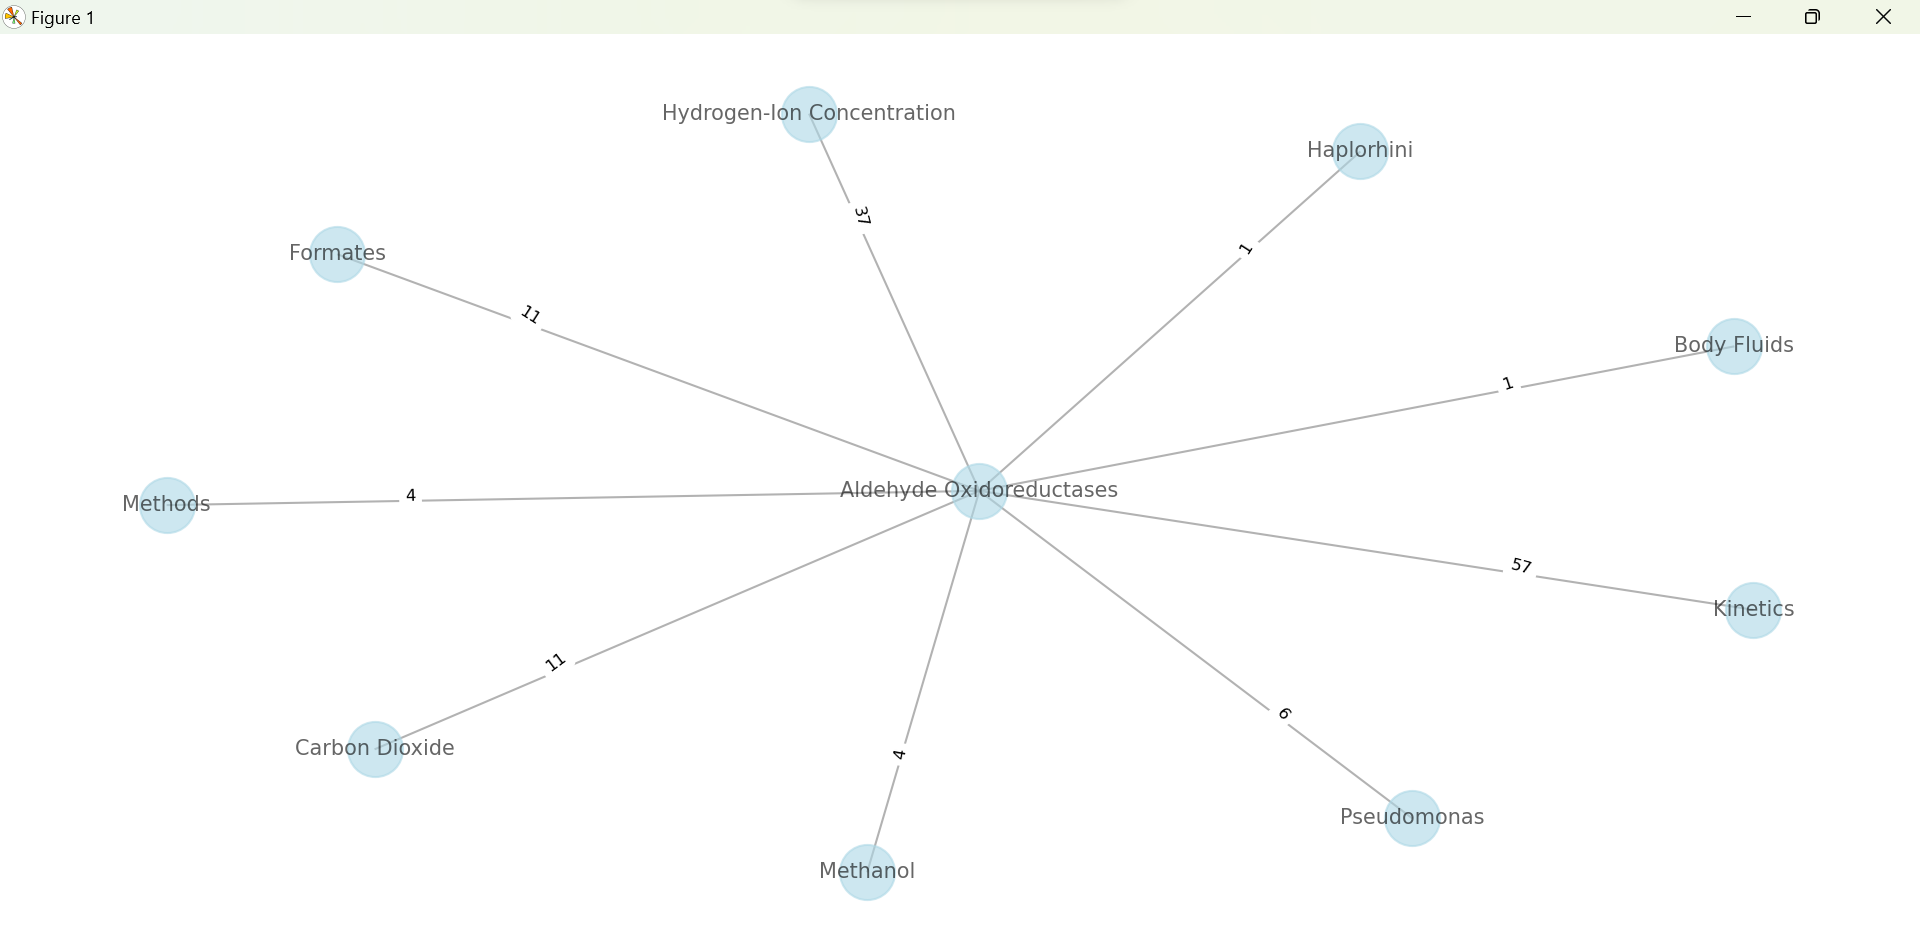
\includegraphics[width=\linewidth]{images/test_graph_creation.png}
    \caption{A small test graph to sanity check the graph creation process.}
    \label{fig:test_graph_creation}
\end{figure}

\subsection{Sub-Graph Creation} 

For all of the subsequent systems I create, I would want to be able to test them on smaller sub-graphs so execution times are faster for testing purposes and to more easily evaluate if they are functioning correctly. However, as can be seen in \Cref{fig:test_graph_creation}, the data when used for creating these graphs is organised by how the pairs of tags were initially ordered in the dataset files. I was concerned that this data trend would continue into the graphs, resulting in strange and unhelpful graphs such as that shown in \Cref{fig:test_graph_creation}. Therefore I ran a test of creating a sub-graph from the before 2008 graph containing ten nodes. This graph can be seen in \Cref{fig:test_subgraph}. As can be observed in this graph, it is much more meaningful and contains more information of the relationships between each of the nodes present than was the case in \Cref{fig:test_graph_creation}. \\

\subsection{Filtering Graphs}

For making and evaluating my link predictions, I required certain features in the data. Firstly, in my post-2008 graph, I only wanted to have edges present that were not present in the pre-2008 graph. That is to say, if the link between concepts A and C had already been established before the time-split, there is no value in predicting it. Furthermore, I only wanted to predict about nodes, or MeSH tags, that I had already seen in the before 2008 graphs. Therefore, I combed through the post 2008 graph and removed any edges that existed in the before 2008 graph and any nodes that did not. This resulted in a filtered post-2008 graph with 362987 edges and 9653 nodes. \\

\begin{figure}[h]
    \centering
    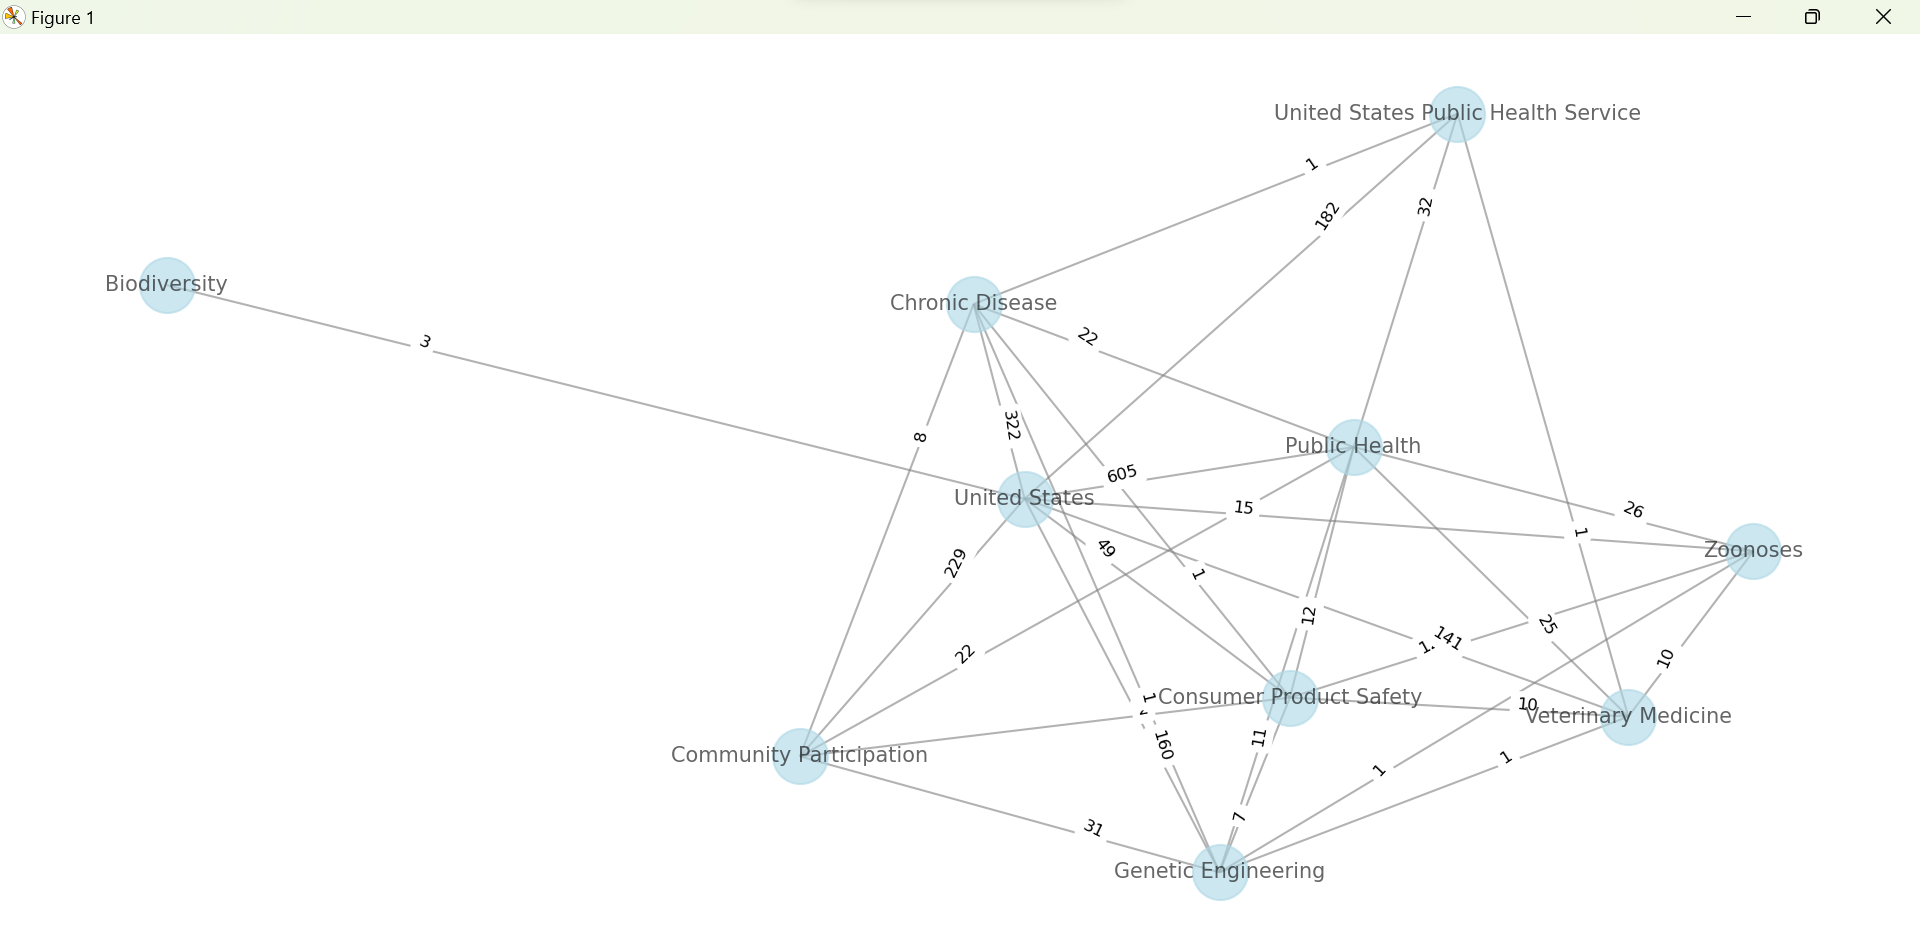
\includegraphics[width=\linewidth]{images/test_subgraph.png}
    \caption{A small test sub-graph to sanity check the sub-graphing process.}
    \label{fig:test_subgraph}
\end{figure}

\section{Swanson ABC}

\subsection{Initial Process}

The first prediction system I implemented was Swanson's ABC system. First, this required for each A node, generating a list of B nodes by returning the neighbours of that A node. At this stage we had the all of the concepts that co-occurred in articles with the MeSH tag represented by that A node. The next step was to get the neighbours of each of these B nodes, however there was an additional stipulation here. These new neighbours had to be filtered for any of the other B nodes. This is because, to qualify as a C node, the node in question must not already be connected to the A node. Once this filtering was done, a set of C nodes and B nodes was complete for each possible A node. \\

\subsection{Sorting C nodes}

As it stands, the system thus far simply returns all possible C nodes with no ability to evaluate how good each of these C nodes is as a prediction of a future link. To evaluate these predictions, they need to be sorted by some system which can rank them. With the data provided by our system there are three ways that these C nodes can be ranked. \\

The first approach is to use the total weight of the edges that connect each C node to the original A node. An easy mistake to make here is to only consider the edges from the C node and sum these. However, the weight of the edges between the A node and the B nodes should also be included here. For example, if $A$ and $C$ are connected by nodes $B_1$ and $B_2$, the total weight of the connection between $A$ and $C$ will be the summed weight of edges $AB_1$, $AB_2$, $CB_1$ and $CB_2$. This can formalised as follows, where $n$ is the number of $B$ nodes that connect $A$ and $C$.
\begin{center}
    $C_{\text{weight}} = \sum_{i=1}^n ((AB_i)_{\text{weight}} + (CB_i)_{\text{weight}})$ \\
\end{center}

The next sorting system will use the number of connecting B nodes between each A and C node. This means that each possible C MeSH tag will simply have a value attributed to it equal to the number of MeSH tags that appear in an article with both it and the original A tag. For example, if A and C are connected by nodes $B_1$ and $B2_$, the C node will be evaluated with a frequency score of 2. This can formalised as follows, where set $B$ is the set of nodes that connect A and C.
\begin{center}
    $C_{\text{frequency}} = |B| $\\
\end{center}

The final method of ranking these C nodes is to combine the previous two systems. To do this I multiplied the two values together. I opted not to sum them together as this would make the frequencies fairly irrelevant in the calculation. This calculation can be formalised as follows, given the previous two equations we have just defined. The only modification made, is that the square root of the value is taken so as to keep the numbers of the same dimensionality and easier to compare.

\begin{center}
    $C_{\text{combined}} = \sqrt{|B|(\sum_i^n ((AB_i)_{\text{weight}} + (CB_i)_{\text{weight}}))}$\\
\end{center}

\subsection{Sanity check}

To ensure that these systems were producing the results I wanted I conducted a ``sanity'' check on them using the small, ten node graph seen previously in \Cref{fig:test_subgraph}. I used the node ``United States Public Health Service'' node as A to evaluate on this graph. This node had five C nodes, giving a range of different frequencies, weights and combined scores. Here are the frequencies as an example of how the C nodes can be sorted. These scores can be checked against \Cref{fig:test_subgraph} to confirm that the system is correctly evaluating the frequencies.\\

\begin{table}[h]
\centering
\caption{Data Sorted by Frequency}
\begin{tabular}{|c|c|c|}
\hline
\textbf{Position} & \textbf{Frequency} & \textbf{Name} \\ \hline
1 & 4 & Genetic Engineering \\ \hline
2 & 4 & Consumer Product Safety \\ \hline
3 & 3 & Community Participation \\ \hline
4 & 3 & Zoonoses \\ \hline
5 & 1 & Biodiversity \\ \hline
\end{tabular}
\end{table}

\section{Graph Neural Network}

\subsection{PyTorch}

PyTorch, created by Facebook AI Research and other labs, blends fast and flexible GPU-accelerated libraries with an easy Python interface. It's an excellent tool for quickly trying out new ideas and works with many types of deep learning models. It allows for coding in python but with the efficiency usually reserved for other more demanding languages. PyTorch is well integrated with other packages such as SciPy, NumPy and NetworkX, enabling seamless and efficient programming. Furthermore, PyTorch is widely used in data science studies and publications thereby enabling for easier collaboration and sharing of research and replication and validation of results. \\

Within PyTorch is a sub library PyTorch Geometric which is designed to allow straightforward creation and training of GNNs for structured data such as graphs. It is this library that contains the aforementioned function that allows for the easy translation from NetworkX graphs to PyTorch Data structures. In addition, it contains a variety of functionalities to allow for deep learning on graphs such as batch loaders, graph convolution networks (GCNs) and GNNs. \\

\subsection{Starting building}

Despite these benefits, I found it incredibly hard to get into PyTorch. Complicated tutorials, dense documentation and endless functions within functions made for a near insurmountable entry to the software. This lead to a lot of time being spent going round in circles without producing anything, just trying to fix bugs within bugs and creating more problems than I was solving. To rectify this spiral, I opted to copy a tutorial from Medium written by Jan Eric Lenssen and Matthias Fey, that builds a link prediction model on a heterogeneous graph. This tutorial follows a PyTorch tutorial on link prediction but adds to it explanations of functions and concepts to aid with development and understanding. \\

Translating this code to fit my data was very challenging. Their \texttt{train\_loader} using the PyTorch Geometric \texttt{LinkNeighbourLoader()} did not accept their data format, and when I tried to fit it to my data, once again did not work there either. Moving forwards with the development, I had to change their data set up to accommodate my graphs. The biggest hurdle in this process was translating it from heterogeneous to homogeneous. I had assumed that this would be a straight forward process given that I would be reducing the required information. However large components of the system were built on the assumption and utilisation of the different aspects of this data. This caused endless problems and seriously slowed down development. Weeks were spent pouring over documentation, changing a couple of lines, re-running code, no change, repeat, some change, new bug, repeat. A serious problem faced was the difficulty in bug fixing PyTorch code due to the black box nature of so many of the core functions. Eventually, a break through enabled the system to train successfully and produce predictions. \\

The next problem faced was the absence of negative sampling. In the tutorial provided, this had been done by the batch loader and the link splitter, a function that divided the data into training and test sets, and so was not used in my system which was already split. This obviously resulted in extreme predictions being made due to the system not seeing any negative data. This was resolved by using the negative sampling function of PyTorch Geometric and adding negatively weighted edges to both the training and the testing data sets. \\

\subsection{Performance Evaluation}

To evaluate the performance of this system I used the area under the curve (AUC) of the receiver operating characteristic (ROC) curve. An ROC curve graphically represents a classification model's performance across different classification thresholds, and is a plot of the True Positive Rate (TPR) against the False Positive Rate (FPR). \\

The TPR is defined as: 

\begin{center}
    $\text{TPR} = \dfrac{\text{TP}}{\text{TP} + \text{FN}}$ \\
\end{center}

\vspace{10mm} 
and the FPR is defined as: 

\begin{center}
    $\text{FPR} = \dfrac{\text{FP}}{\text{FP} + \text{TN}}$
\end{center}

where TP represents the true positives, FN represents the false negatives, FP represents false positives and TN represents true negatives. An ROC curve depicts the relationship between TPR and FPR across various classification thresholds. Decreasing the classification threshold results in more items being classified as positive, thereby elevating both False Positives and True Positives. \\ 

\begin{figure}[h]
    \centering
    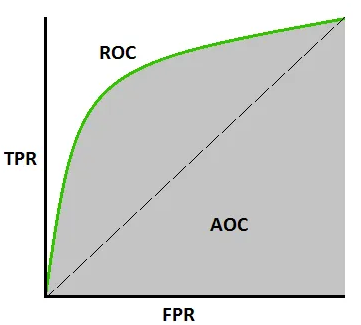
\includegraphics[width=0.5\linewidth]{images/roc_auc.png}
    \caption{Example of an ROC curve (in green) and the AOC shown in grey. This image is taken from the webpage: \href{https://towardsdatascience.com/understanding-auc-roc-curve-68b2303cc9c5}{\textcolor{blue}{understanding-auc-roc-curve}}}
    \label{fig:roc_auc}
\end{figure}

To evaluate what the graph shown in \Cref{fig:roc_auc} indicates, we use the AUC, which implies that the chance that a true example would be evaluated by the model as higher than a false example. The AUC varies between 0 and 1, where an AUC of 0.0 signifies a model with predictions entirely incorrect, while an AUC of 1.0 denotes a model with predictions entirely correct. AUC is advantageous for two primary reasons: It assesses the ranking quality of predictions rather than their absolute values, and it also evaluates the model's prediction quality regardless of the chosen classification threshold. \\

\subsection{Performance Improvement}

The GNN system that I had built now faced a performance problem, it was not very good. Not only was it not very good, it was not better than randomly guessing. On multiple runs the AUC hovered around 0.5, which is to say it has a 50-50 chance of guessing correctly if a link exists or not. \\

To try to improve this performance I systematically walked through fine tuning my hyper parameters. For my GNN. the three hyper parameters that I varied were:
\\
\begin{itemize}
    \item \textbf{Epochs}, the number of cycles that the system iterates over the training data.
    \item \textbf{hidden Channels}, the number of hidden units within the GNN.
    \item \textbf{Learning Rate}, The step size at each iteration that the model makes towards a minimum loss function.\\
\end{itemize}

In the first round of optimisations, I experimented by altering the epochs the number of hidden channels. For each combination of values across these two hyper parameters, I ran five iterations of the system. Displayed in \Cref{tab:Optimisation_results} are the mean and standard deviation across these five results for each combination. \\

\begin{table}[h]
    \centering
    \caption{Optimisation results}
    \label{tab:Optimisation_results}
    \begin{tabular}{|c|c|c|c|c|}
        \hline
        \textbf{Epochs} & \textbf{Hidden Channels} & \textbf{Learning Rate} & \textbf{Run Mean} & \textbf{Standard Deviation} \\ \hline
        5 & 32 & 0.001 & 0.5026 & 0.0044 \\ \hline
        10 & 32 & 0.001 & 0.5044 & 0.0080 \\ \hline
        3 & 32 & 0.001 & 0.5057 & 0.0101 \\ \hline
        5 & 64 & 0.001 & 0.5052 & 0.0075 \\ \hline
        10 & 64 & 0.001 &0.5011 & 0.0041 \\ \hline
        3 & 64 & 0.001 & 0.4947 & 0.0074 \\ \hline
        5 & 128 & 0.001 & 0.4985 & 0.0073 \\ \hline
        10 & 128 & 0.001 & 0.4983 & 0.0083 \\ \hline
        3 & 128 & 0.001 & 0.4976 & 0.0045 \\ \hline
        5 & 16 & 0.001 & 0.5082 & 0.0108 \\ \hline
        10 & 16 & 0.001 & 0.4959 & 0.0052 \\ \hline
        3 & 16 & 0.001 & 0.4964 & 0.0051 \\ \hline
    \end{tabular}
\end{table}

The mean of the standard deviations is 0.0069 and the mean of the means is 0.5007. From this we can take that almost every mean falls within the average standard deviation from the average mean. The only one outside of this range is with 5 epochs and 16 hidden channels with a mean of 0.5082. However this combinations own standard deviation is the largest at 0.0108, which means we cannot reliably say that it is a better combination than any other.\\

Notably in the previous experiment, I did not vary the learning rate. I wanted to take the most interesting and promising combinations from the results displayed in \Cref{tab:Optimisation_results} and then vary the learning rate across these. This was done to reduce the time doing endless repetitions on combinations that were already under performing. The three that I progressed with were as follows. Firstly, the already mentioned 5 epochs and 16 hidden channels for the already discussed reasons. Secondly, 5 epochs and 32 channels was chosen due to its very low standard deviation in the hope that it would be more consistent. 10 epochs with 64 hidden channels had slightly less standard deviation but a lower mean and so was not selected. Finally, the combination of 5 epochs and 54 hidden channels was used due to it having a fairly high mean of 0.5052 but a much lower standard deviation than the first combination at 0.0075. \\

\begin{table}[h]
    \centering
    \caption{Learning rate results}
    \label{tab:Learnng_rate_results}
    \begin{tabular}{|c|c|c|c|c|}
        \hline
        \textbf{Epochs} & \textbf{Hidden Channels} & \textbf{Learning Rate} & \textbf{Run Mean} & \textbf{Standard Deviation} \\ \hline
        5 & 32 & 0.01 & 0.4941 & 0.0099 \\ \hline
        5 & 16 & 0.01 &  0.4975 & 0.0079 \\ \hline
        5 & 64 & 0.01 & 0.4920 & 0.0040 \\ \hline
        5 & 32 & 0.001 & 0.5026 & 0.0044 \\ \hline
        5 & 16 & 0.001 & 0.5082 & 0.0108 \\ \hline
        5 & 64 & 0.001 & 0.5052 & 0.0075 \\ \hline
        5 & 32 & 0.0001 & 0.4963 & 0.0064 \\ \hline
        5 & 16 & 0.0001 & 0.5004 & 0.0185 \\ \hline
        5 & 64 & 0.0001 & 0.4961 & 0.0114 \\ \hline
        5 & 32 & 0.00001 & 0.4993 & 0.0109 \\ \hline
        5 & 16 & 0.00001 & 0.4982 & 0.0123 \\ \hline
        5 & 64 & 0.00001 & 0.5043 & 0.0083 \\ \hline
    \end{tabular}
\end{table}

From these results seen in \Cref{tab:Learnng_rate_results} we can see that three of the four highest means are from the original learning rate of 0.001. The only other mean in that group had a learning rate of 0.00001 and a mean of 0.5043 that puts it third. Accordingly, we can say that the original learning rate of 0.001 is the best to progress with. Despite that, the average standard deviation for this experiment is 0.0094, much higher than the last experiments 0.0069. This tells us that the variations in learning rate resulted in more extreme disparities in results. The average mean for these results is 0.4995, slightly below the mean of the last experiment. \\

Going forwards from these results, I opted to use the most outstanding combination of 5 epochs, 16 hidden channels and 0.001 learning rate, as compared to the rest this combination had performed best. That said, non of these results had significantly improved the system, indicating that the under performance of the system is either due to the data not having any useful signals, or the GNN having some other systemic issues within it. \\

Another system I tried to implement was early stopping. Early Stopping is a regularization method employed in deep neural networks, which halts training when further parameter updates fail to yield improvements on a validation set. It is used to prevent over-fitting without losing model learning. This is done by measuring the loss on the validation set as well as on the training set. Initially this loss will be decreasing as the system trains, however, when the system starts to over fit to the training set the loss on the validation set should start to increase. At this point the training of the system should be halted to prevent over-fitting. I implemented this system on my model, however it also did not make any meaningful changes. \\
\subsection{Sanity check}

Evidently from the results in the previous section, there could be some underlying issues with the system I have created. To try and diagnose the problems facing this system I conducted some sanity checks to understand what was happening. \\

The first thing I wanted to check was if the system could train to completely over-fit on a data set. Over-fitting in machine learning is when a model trains too much on a dataset, and therefore predicts that all other data must look exactly like the training set and anything else is wrong. \\

To do this I created a simple dataset with eight positive edges and four negative edges. I set this dataset as both the training and the testing dataset. With this in place I then ran it at a number of different epoch numbers. First at the normal five it had barely learnt it and gave back a AOC of 0.333. Next, at 100 epochs, it produced a much improved AOC score of 0.71875. Finally at 200 epochs it produced a perfect AOC score of 1.0. This proves that the system can indeed learn from the data and perfectly over-fit a data set. However, a result here that really shocked me was how many epochs it took to learn this. I had expected that by 100 epochs, 20 times the normal amount, it should have learnt such a small dataset completely. This lead me to question, why on each pass of an epoch over the dataset was it learning so little. \\

\begin{figure}[h]
    \centering
    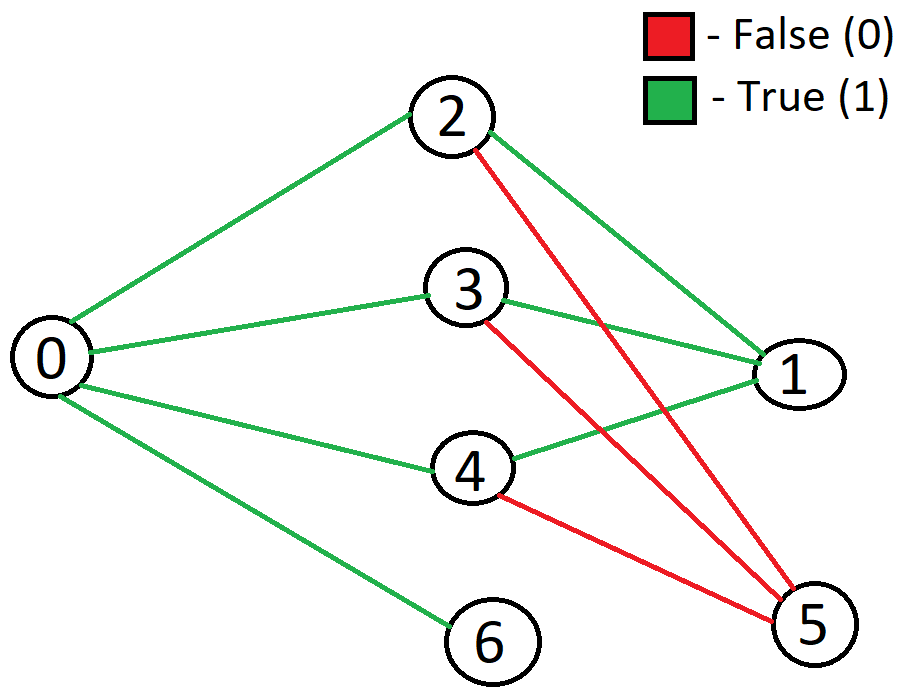
\includegraphics[width=0.5\linewidth]{images/sanity_graph.png}
    \caption{Simple graph to test sanity of system}
    \label{fig:sanity_graph}
\end{figure}

The other sanity check I ran on this system was can it predict obvious missing links. To measure this I gave it a simple graph with clear patterns as can be seen in \Cref{fig:sanity_graph}. Here, the intention is that the GNN should recognise that node 6, if connected to node 0, should also be connected to node 1 and should not be connected to node 5. I ran this system at five epochs, 100 times to see if it would randomly guess the result or could understand the implications of the graph. The average AUC score over 100 iterations was 1.0. The GNN could perfectly understand the obvious missing links and predict what they should be every time. \\

Therefore, these results indicate that the system is sane, it can over-fit to data it has seen before, given enough epochs, and it can predict obvious missing links consistently from simple graphs. However, there is still something strange happening. It seems to take the system a lot longer than it should to fit the data that it is seeing. This would imply that somehow, on an epoch to epoch basis, it is learning very slowly and not gaining much understanding of the data. \\

To test if this system is just learning really slowly, I ran it with 500 epochs. This resulted in it giving me a AUC score of 0.5357, which is much higher than previous runs. This would indicate that it had learned from the data better at 500 epochs than it had at five. At 1000 epochs it went back down to 0.5175, which tells that at some stage between here and 500 the system started over fitting. At this point I was very late on in my project and did not have the time available to be able to fix this problem. I believe that the solution to this problem lies in figuring out how to get batching and data loaders working for this system. I had some tinkering with this but failed to make it work and so had to move on. \\

\subsection{Final Parameters}

Due to these experiments and checks, the resulting GNN system to be used in answering my research will have the following features; 64 hidden channels, learning rate of 0.001 and 500 epochs. However, the system could not run on the machine available on the full graph, so a subgraph of 1000 nodes and 176826 edges in the training set and 13084 edges in the test set.\\

\section{Matrix Factorisation}

\subsection{Starting Building}

Having learnt lessons from the implementation of the GNN, I began my implementation of the matrix factorisation system by following a tutorial. For this I followed the precess published in a blog post by Ethan Rosenthal \textcolor{red}{[ref]} recommended to me by my supervisor. Ethan had previously made posts about how to implement the matrix factorisation algorithms manually, but this post used the tools that PyTorch provide to make the whole process much simpler and more straightforward. \\

This implementation also faced issues and bugs, but with the experience of related problems with the GNN I was able to more easily overcome them. In particular I encountered problems of the system being designed for heterogeneous data, but this time I was able to resolve this issues more quickly thanks to my prior experiences. A key benefit of this system, as compared to the GNN, was it was much less complicated and more straightforward. This, combined with the lessons learned, enabled me to swiftly break through many of the issues including adding in negative sampling, designating node ids and evaluating performance. \\

\subsection{Performance Improvement}

Once working, the matrix factorisation faced similar problems to the GNN with its AUC score being close to 0.5. Therefore I conducted a similar experiment with the hyper parameters as with the GNN analysis. For this system at this point the hyper parameters I had to change were learning rate and hidden channels, which are termed vector factors. With these variables I re-ran the tests which resulted in it being clear that 64 vector factors and a learning rate of 0.001 worked best. However, despite this combination performing best, it still only had a mean AUC score of 0.5021, which is very close to random guessing. \\

I discussed these results with my supervisor, who recommended a set of changes to improve the system. First of these was running for multiple epochs, he realised that the system I had built at this stage was not doing this obvious step. Secondly, my system was adding negative edges by concatenating them onto the positive edges. This meant that when the system walked through all the edges it would see all the positive edges and then all the negative edges. The consequences of this might be that this does something strange to the model calculations and throws it off. Therefore, the proposal was to use a data loader to shuffle the edges. An additional benefit of this data loader is that I could use it to also introduce batching to my system, a common practice in deep learning to help handle large datasets. Finally, he also recommended changing the loss function. I was using the same system as was used in the tutorial, MSELoss, but this function is used for non-binary classification. Therefore I switched over to the same system as my GNN, binary cross entropy. Binary cross entropy is the standard method of calculating loss in deep learning in binary systems and so therefore is mnore appropriate fit for this model.\\

At this stage I should have conducted another round of hyper parameter optimization tests, particularly experimenting with batch sizes and epochs. However it was very late on in the project, and I did not have time. Conducting these experiments could have improved the system to some extent, but would unlikely to have significantly improved the system. \\

I implemented each of these systems into my matrix factorisation model successfully. However, when I ran my system again with these changes, it still was performing around an AUC of 0.5. Therefore, I once again went on to conduct a sanity check to understand what was happening with my system. \\

\subsection{Sanity check}

As with the GNN the first experiment in the sanity check was testing if the system could over-fit on a graph and predict it perfectly. When ran at only five epochs, the system did not perform very well at all. However, when ran 100 times at 50 epochs, it averaged an AUC score of 0.995. This demonstrates that given enough time, this system can over-fit and learn a training set near perfectly. At a 100 epochs, it was then scoring an average of 0.999, which is pretty much perfect. Interestingly, at neither of these thresholds did it get it right every single time, which indicates that this system still was not quite getting a perfect understanding of this data even at this many epochs. \\

The second step of the sanity check was to measure the ability of the system to predict missing edges on an obvious graph. To do this I used the same graph as I did with my GNN, shown in \Cref{fig:sanity_graph}. I conducted this experiment again 100 times at the base epochs of five, resulting in a perfect AUC score across these runs of 1.0. This successfully demonstrates the my system can predict obvious edges and learn from the training set about trends in the data. Therefore, we can conclude that the system is sane as it can predict both obvious missing edges, and over-fit to a training set. \\

\subsection{Final Parameters}

Due to these experiments and checks, the resulting matrix factorisation system to be used in answering my research will have the following features; 64 vector factors, learning rate of 0.001, shuffled edges, five epochs and binary cross entropy loss function. \\

\chapter{Evaluation} 

\section{Research Question 1}

The first research question (RQ) is, how do link weight and link count compare and the combination of these compare in an ABC prediction system using a MeSH tag knowledge graph? To answer this I used Hits@K to evaluate and compare three different sorting systems; weight of edges, number of edges, combination of weight and number of edges. \\

\subsection{Hits@K}

Hits@K is the evaluation method used to measure the prediction capabilities of these different sorting systems. Hits@k evaluates the accuracy of predicted links in knowledge graphs for missing link prediction by assessing the model's ranking of true versus false missing links. It gauges the percentage of correct predictions within the top k ranked links, with a higher Hits@k value signifying superior performance in missing link prediction. This assessment method is widely employed in link prediction tasks to gauge the efficacy of various models and algorithms. \\

\subsection{Process}

To compare the three approaches I will evaluate them across four k values, one, five, ten, and twenty. These values will be calculated from making predictions across 100 nodes and averaging the results. The data used for this experiment will be the standard 1000 node sub graph which is used in other experiments in this paper due to the limitations imposed by the GNN.\\

\subsection{Results}

\begin{table}[h]
    \centering
    \caption{RQ1 Results}
    \label{tab:rq1_results}
    \begin{tabular}{|c|c|c|c|}
    \hline
    & \textbf{Weight Only} & \textbf{Count Only} &\textbf{Weight and Count} \\ \hline
    \textbf{K value} & \textbf{Hit Rate} & \textbf{Hit Rate} & \textbf{Hit Rate}\\ \hline
    1 & 0.17 & 0.2 & 0.19 \\ \hline
    5 & 0.162 & 0.202 & 0.164\\ \hline
    10 & 0.16 & 0.192 & 0.166 \\ \hline
    20 & 0.145 &0.1655 & 0.146\\ \hline
    Mean & 0.159 & 0.19 & 0.167 \\ \hline
    \end{tabular}
\end{table}

\subsection{Discussion}

The results from this experiment can be seen in \Cref{tab:rq1_results}. From these findings there is a clear best approach. Using count not only performed best overall, but also across every single K value. Weight only was the approach which had the worst performance with the combination of the two sitting between them. Interestingly, the combination of the two performed much closer to weight only than to count only. This would indicate that the weight has a significantly greater effect on this system than the counts do, and so warps the results closer to weight only. \\ 

Therefore, the answer to this research question is that edge count is a better metric to use in link prediction on this data set than link weight or a combination of these two. \\

\section{Research Question 2}

The second research question (RQ) is, how do the ABC, GNN, and matrix factorisation systems compare to each other, when predicting on a MeSh tag knowledge graph? To compare these systems I ran all three on a common data set and evaluated them all with AUC score and my own system of evaluating their top scoring edges in the predictions. \\

\subsection{Data}

Each of these systems were trained on the same data set. A sub-graph of 1000 nodes taken from the pre-2008 graph, the same as used in RQ1 (and later for RQ3). this ensures that each system was given the same information for learning about the data so as to create a level playing field with more comparable results. Using a reduced set of the data was necessitated by the memory limits of my machine when running the GNN. \\

The test data set was carefully curated to produce a reduced data set that could then also be used in RQ3 so as to allow the results data to be comparable between the two experiments. I wanted to measure how well these systems could perform on nodes for which there is a lot of information ind in particular nodes that have many edges in the pre-2008 set, and also have many positive edges in the post-2008 data set. This would allow me to evaluate how these systems perform when given meaningful information to work with and a significant prediction tarrget. \\

To do this, I sorted the both graphs by how many edges each node has, the degree of that node. I walked through the top 100 degree nodes on each graph to find nodes were in common between them. For each of these nodes, I constructed a graph containing all the edges from that node to nodes that were non-existent in the pre-2008 graph. This meant that each graph was overwhelmingly more negative than positive in edges. However, this was still the best ratio I could produce this way out of the nodes in the graph. \\ 

The result of this was across three runs, six graphs were created each time, with an average of 299 total edges and nine positive edges within each. \\

\subsection{Metrics}

The first metric I used to compare the performance of these systems against each other was the previously introduced AUC score. Since this is a well established metric used across deep learning research, it makes sense to use as a metric that can be easily understood by readers and compared to other research. The second metric I used is one of my own creation. My main motivation for using it is it is a better way to evaluate the combination of systems in RQ3. However I also used it here, as it can be used to compare the systems individually so as to give further context to my discussion of results in RQ3. \\ 

The secondary metric is similar in concept to the Hits@K metric previously discussed. It represents how well in a top k number of values has the system predicted positive results. Instead of representing this value as a ratio of those k values, it calculates the ratio of positive results in the data set as a whole and compares to this. Therefore, if the system is randomly guessing, a score of 1.0 would be expected, as for each positive result expected in the k terms, the system produces one. A score less than 1.0 indicates that the system is worse than randomly guessing, and is somehow systematically ranking positive values lower than negative ones. On the other hand, a score greater than 1.0 indicates that the system is ranking positive results on average higher than a random guessing system would. The score value, at any level, will give a simple comparison to a randomly guessing system. A score of 2.0 means the system is twice as good as a random one, and a score of 0.5 means the system is half as good as a randomly guessing system. This can be represented as follows.\\

\begin{center}
    $\text{Score} = \dfrac{\left ( \dfrac{\text{Correct Guesses}}{\text{Total Guesses}}\right )}{\left ( \dfrac{\text{Positive values}}{\text{Total values}}\right )}$ 
\end{center}

The purpose of evaluating only the top k guesses, is because this is a prediction system. The user is not interested in the bottom ranking values, but only in the ones that are highest ranked by the system. It is intended to be used for discovery of possible links between concepts. Therefore the highest ranking edges in the prediction are the ones of most value to the user, and so the ones most worth evaluating. \\

These relative scores will be calculated for k-values 1, 10, 20, 50, and 100 so as to provide insight at a range of cuts from the predictions. \\

\subsection{Results}

\begin{table}[h]
    \centering
    \caption{RQ2 AUC score}
    \label{tab:rq2_auc}
    \begin{tabular}{|c|c|c|c|c|}
    \hline
    & \multicolumn{3}{|c|}{AUC Scores} & \\ \hline
    \textbf{System} & \textbf{Run 1} & \textbf{Run 2} & \textbf{Run 3} & \textbf{Mean}\\ \hline
    ABC & 0.778 & 0.735 & 0.617 & 0.710 \\ \hline
    GNN & 0.671 & 0.557 & 0.547 & 0.592 \\ \hline
    Matrix Factorisation & 0.556 & 0.543 & 0.400 & 0.500 \\ \hline
    \end{tabular}
\end{table}

\begin{table}[h]
    \centering
    \caption{RQ2 Relative Score Averages}
    \label{tab:rq2_rsa}
    \begin{tabular}{|c|c|c|c|c|c|c|}
    \hline
    & \multicolumn{5}{|c|}{K value} & \\ \hline
    \textbf{System} & \textbf{1} & \textbf{10} & \textbf{20} & \textbf{50} & \textbf{100} & \textbf{Mean}\\ \hline
    ABC & 10.36 & 3.99 & 3.36 & 2.40 & 1.85 & 4.39\\ \hline
    GNN & 3.11 & 3.07 & 2.38 & 1.42 & 1.36 & 2.27\\ \hline
    Matrix Factorisation & 1.26 & 1.09 & 1.21 & 0.78 & 0.91 & 1.05\\ \hline
    Mean & 4.91 & 2.72 & 2.33 & 1.53 & 1.37 & \\ \hline
    \end{tabular}
\end{table}

\subsection{Discussion}

Firstly, the AUC scores in \Cref{tab:rq2_auc} paint a very clear picture of the three systems. The ABC system comfortably out performed the other systems with an average score of 0.71, which is higher than any other system's highest score. Another interesting phenomenon in these results is that all three of them performed best on run 1 and worst on run 3. This means that as one system finds a graph more difficult to predict, so to do others, indicating that they might be evaluating them using similar metrics. The purpose of building the machine learning systems is that despite taking longer to train, they are supposed to be able to out-perform traditional algorithmic systems like ABC. However it is clear that for this test set this has not been achieved for reasons that are not clear. This culd be that the training and test set were too small to allow the power of machine-learning to be realised. Trailing in last place was matrix factorisation which only just broke even with a randomly guessing system in AUC score. \\

The trends seen in the AUC scores are supported in the relative scores \Cref{tab:rq2_rsa}. Once again, the ABC system performs best on average and the matrix factorisation system is worst, being very close to a randomly guessing system. Some interesting outliers in these results, such as the ABC system having a score of 10.36 at a k-value of 1. On further exploration of this result I found that of the 18 different graphs it evaluated, the edge it ranked top was right, five times, as compared to only once by each of the other two systems. This makes for a rather exaggerated relative score, but is still very useful as the top returned result is the one that researchers will be most interested in. As the k value increased, so to did the relative scores decrease on average. This could be due to two possible reasons, the data sample is getting larger and so maybe the metric is normalising closer to how the systems are actually performing, or it could be that the systems are better at guessing the more obvious edges than getting the more difficult shouts right, and so perform better if a smaller number of the results are used for evaluation. If the first of those two is true we would expect to see, among the smaller k-values, results both above and below the scores at larger k-values. However, it is a fairly consistent decrease as the k-values increase, indicating that the second of the two possibilities is more plausible. \\

To answer the research  question, both metrics conclude that ABC is the best of the three systems, and that matrix factorisation is, not only the worst, but also not any better than a randomly guessing system. \\

\section{Research Question 3}

The third research question (RQ) is, How do the various possible combined use of the ABC, GNN, matrix factorisation systems compare to each other and to these systems individually? Between these three systems there will be four combinations, ABC and GNN, GNN and matrix factorisation, matrix factorisation and ABC, and all three of them combined. I will use the same secondary system I used to evaluate RQ2 to compare these systems to each other and to the individual systems. \\

\subsection{Data}

Once again, each of these systems were trained on the same data set of a sub-graph of 1000 nodes taken from the before 2008 graph, the same as used in RQ1 and RQ2. For the test data, the same set of node graphs were created and used as in RQ2. Across the three runs of this evaluation, six graphs were created each time, with an average of 299 total edges and 12 positive edges each. \\

\begin{figure}[h]
    \centering
    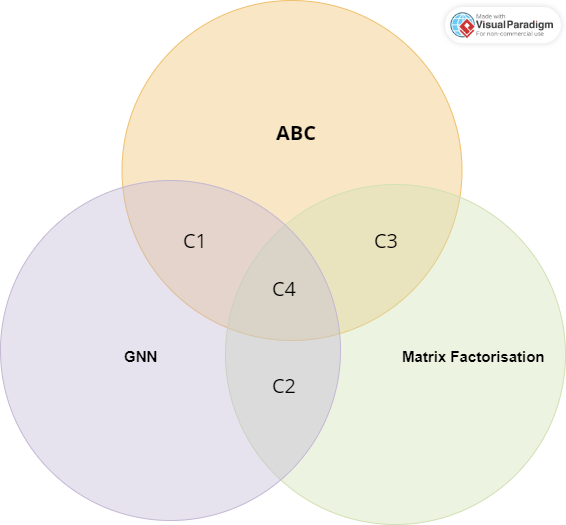
\includegraphics[width=0.6\linewidth]{images/Combination_venn.png}
    \caption{Venn Diagram of system combinations}
    \label{fig:venn}
\end{figure}

To get the combined prediction of these systems, I took, for each k-value, the common ground or \textit{intersection} of the predictions from each the systems within a particular combination. I labelled each of these combinations C1 to C4, as can be seen in \Cref{fig:venn}. Score predictions of each predicted edge were not combined between system because the ABC system scored edges very differently to the other two, which would create an unbalanced combination measure as seen in the results of RQ1. Therefore, the overlap between the top k predictions was taken instead, which further enhances the performance of the systems being used as discovery systems. \\

\subsection{Metrics}

Because of the vastly reduced datasets caused by only taking the overlap of the top k predictions, an overall evaluation using AUC is no longer useful. Therefore, the only metric that will be used to evaluate these combinations is the relative score metric defined in for RQ2. These values will be calculated for k-values 20, 50, and 100 as 1 and 10 will return so few overlapping values that they will not provide any meaningful data.\\

\subsection{Results}

\begin{table}[h]
    \centering
    \caption{RQ3 Average Edges in common}
    \label{tab:rq3_common}
    \begin{tabular}{|c|c|c|c|}
    \hline
    & \multicolumn{3}{|c|}{k value}\\ \hline
    \textbf{System} & \textbf{20} & \textbf{50} & \textbf{100} \\ \hline
    C1 & 5.056 & 18.722 & 50.111  \\ \hline
    C2 & 1.556 & 9.111 & 35.111\\ \hline
    C3 & 1.556 & 8.389 & 34.111\\ \hline
    C4 & 0.556 & 3.722 & 18.055\\ \hline
    Mean & 2.181 & 9.986 & 34.347\\ \hline
    \end{tabular}
\end{table}

\begin{table}[h]
    \centering
    \caption{RQ3 Average Edges Correct}
    \label{tab:rq3_correct}
    \begin{tabular}{|c|c|c|c|}
    \hline
    & \multicolumn{3}{|c|}{k value} \\ \hline
    \textbf{System} & \textbf{20} & \textbf{50} & \textbf{100}\\ \hline
    ABC & 1.611 & 3.722 & 6.444 \\ \hline
    GNN & 1.333 & 3.167 & 5.389 \\ \hline
    Matrix Factorisation & 0.722 & 2.111 & 4.556 \\ \hline
    C1 & 0.5 & 1.556 & 3.778 \\ \hline
    C2 & 0.167 & 0.556 & 1.833 \\ \hline
    C3 & 0.111 & 0.444 & 2.167 \\ \hline
    C4 & 0.111 & 0.333 & 1.333 \\ \hline
    Mean & 0.650 & 1.698 & 3.643 \\ \hline
    \end{tabular}
\end{table}

\begin{table}[h]
    \centering
    \caption{RQ3 Average Relative scores}
    \label{tab:rq3_score}
    \begin{tabular}{|c|c|c|c|c|}
    \hline
    & \multicolumn{3}{|c|}{k value} & \\ \hline
    \textbf{System} & \textbf{20} & \textbf{50} & \textbf{100} & \textbf{Mean}\\ \hline
    ABC & 2.219 & 1.886 & 1.604 & 1.903\\ \hline
    GNN & 1.582 & 1.456 & 1.286 & 1.44\\ \hline
    Matrix Factorisation & 0.858 & 1.001 & 1.079 & 0.979\\ \hline
    C1 & 1.792 & 1.709 & 1.892 & 1.798\\ \hline
    C2 & 1.452 & 1.358 & 1.188 & 1.333\\ \hline
    C3 & 0.800 & 1.232 & 1.437 & 1.156\\ \hline
    C4 & 1.534 & 1.859 & 1.631 & 1.675\\ \hline
    Mean & 1.463 & 1.500 & 1.445 & \\ \hline
    \end{tabular}
\end{table}

\subsection{Discussion}

First, to put in context all of the results we first examine the three systems on their own. In \Cref{tab:rq3_score}, we can see that once again, ABC has performed best and matrix factorisation is worst and is basically randomly guessing. These three systems are not included in \Cref{tab:rq3_common} as they will always have the full k-values. This is also why in \Cref{tab:rq3_correct} the three systems have massively more correct edges in their selection, simply due to the difference in total edges. \\

Looking at \Cref{tab:rq3_common}, we can see that at almost every value of k, every system had less than half of their edges in common with each other and often, significantly less. The biggest reduction was C4, which is all systems combined, with a k-value of 20 going down to 0.556 edges on average which is less than 3\% of an overlap of 20. As k increases, so to does the proportion of edges in common between systems. This would mean that the top few ranked edges by each of these systems are very rarely the same, which tells us that, despite similar trends between systems on each run seen in RQ2, the top ranked predictions rarely match. \\

Examining the scores themselves in \Cref{tab:rq3_score}, there are a few interesting trends to identify. Firstly, the influence of matrix factorisation on any combination is clearly negative. In particular, the common ground between matrix factorisation and ABC is particularly bad, despite the ABC system performing best. Even the combination combination of GNN and matrix factorisation is better, perhaps because their prediction systems have more in common. \\

The best performing combination is C1, or the GNN and ABC overlap. This is not particularly surprising given that these are the best two systems, however, as seen when comparing C3 and C4, the quality of the individual systems does not necessarily define the quality of the overlap. Not only is C1 the best combination, but at a k-value of 100, it is the best system overall. This is an interesting phenomenon, where the combination of these two systems has not resulted in an averaging of them but instead, an improving on their individual predictions. At this value, C1 meaningfully reduces the total edges from 100 to 50, and increases the quality of these 50 by increasing the hit rate of these edges as compared to other systems. \\

Overall, the best performing system on average is the ABC system and so none of the combinations can be said to be clear improvements on it. However, this is largely influenced by its score at a k-value of 20, the smallest data set and so the least meaningful result accordingly. An interesting system to examine further is C4, the combination of all three systems, taking only edges found in all of their top k results. The expectation would be that this system gets dragged down by matrix factorisation and fails to compete with either ABC or C1 on score. However, at a k-value of 50, it performs almost as well as the top system, ABC, and is clear of any other system, individual or combined. Furthermore, with a k-value of 100, this system performs better than any of the individual systems, but is ultimately not able to match C1. At this k, it seems to benefit from the additional value generated by C1, but then loses some of it when having to involve matrix factorisation. \\

\chapter{Conclusion}    

\section{Summary}

With this project I successfully examined some aspects of using MeSH tags for literature based discovery. I created a knowledge graph representing the co-occurrence of the tags in articles. This stage of the process went smoothly, and resulted in the desired outcome without any problems. \\

The next of this project was the implementation of the three systems. Once again, the implementation of the ABC system went smoothly, but issues started to arise with the GNN. A lot of time was lost in this project in trying to learn and work with PyTorch. If doing this project again I would make sure to start learning and practicing with PyTorch from much earlier in development to allow for this stage to go more smoothly. Another mistake I made at this stage of the project was conducting my fine tuning before my sanity checks. Because of this, the findings from the sanity checks could not be implemented into the fine tuning tests, and so the results from the hyper parameter tuning lost some relevance and accuracy. \\

The evaluations conducted for the research questions produced the necessary results to deliver a meaningful answer to each question within the reduced dataset could be used with the compute hardware available. Evaluation of the ABC system enabled us to learn that the \textit{number} of articles that two tags appear in together is no more useful than the fact there is a link (i.e. each link should have a weight of 1) as information for the ABC system to use when making predictions. When comparing the three systems against each other, both metrics provide the conclusion that the ABC system performs best and the matrix factorisation is the worst. This is a good sign for the use of MeSH tags for LBD, as it should be possible to create a machine learning system that outperforms a simple algorithm like this. The results from the combination of the three systems did not however deliver clear conclusions on which combinations if any would improve performance. While the combinations, in particular the union of the ABC and GNN systems, did not outperform the ABC system, they did manage to perform better than just the average of the two systems individually. Therefore, combining such systems could well be an interesting avenue of research. \\

\section{Future Work}

There are several interesting ways this research can be taken further. First of all, utilising the tree structure of the MeSH tags to automatically assign additional information to the graph could be an excellent way to develop the data. Using this system it should be possible to accurately identify nodes that are drugs, chemicals or diseases among others. Furthermore, once nodes have been have been categorised this way, edges could then be labelled according to the relationship that they represent between the nodes. This would result in a heterogeneous graph and so would also require changing all of the systems to utilise the additional information in their training and prediction processes. \\

Given the performance of the ABC system in comparison to the GNN, I believe that it should be possible to significantly develop this system. Given more time to tinker with the system, and more experience with PyTorch when doing so, the performance of such a system should be able to eclipse the ABC system. \\

If these two can both be done, then, with appropriate resources, they could well be combined to create an LBD system that can be compared to other research in the field. This would then pull together this exploration of using MeSH tags for LBD. \\

\begin{appendices}

\chapter{Appendices}

There are no appendices. 

\end{appendices}

%==================================================================================================================================
%   BIBLIOGRAPHY   

% The bibliography style is abbrvnat
% The bibliography always appears last, after the appendices.

\bibliographystyle{abbrvnat}

\bibliography{l4proj}

\end{document}
